\Large

{\sffamily\Large\bfseries What will you learn in this class?}

You will learn how to write programs that run fast and use computers
efficiently.

If you have a computation-heavy problem that you would like to go
faster, you're especially welcome.

\begin{comment}
\textbf{Pop Quiz:} \$400 at your favorite electronics retailer
buys you a parallel computer that will do
$4\cdot 10^{12}$ floating point operations (``flops'') per second,
but only load $5\cdot 10^{10}$ values from memory in the same
amount of time. How do you use such a machine well?
\end{comment}

\vspace{2.5ex}
{\sffamily\Large\bfseries What to expect}
\vspace{-1.5ex}
\begin{itemize}
\setlength{\itemsep}{-1mm}
  \item Basic processor architecture
    Performance of sequential code
  %\item Why go parallel? Forms of parallelism
  \item Shared Memory and \textbf{OpenMP}
  \item Distributed Memory and \textbf{MPI}
  \item \textbf{GPUs} and \textbf{OpenCL}
  \item Tools and Debuggers
  \item Examples drawn from numerical linear algebra and numerical
    methods for PDEs
  %\item Common Patterns in Parallel Algorithms
\end{itemize}

Class and homework assignments will be based on C.
(warm-up provided for those coming from
Java or Fortran)

\emph{Assessment:} Weekly homework, final
project. (recommended even if auditing)

We're looking forward to seeing you in the fall!
\vspace{1.5ex}

\hfill
\begin{minipage}{0.4\columnwidth}
  \raggedright
  \emph{Marsha Berger}
  \small\texttt{berger@cims.nyu.edu}
\end{minipage}
\hfill
\begin{minipage}{0.5\columnwidth}
  \raggedright
  \emph{Andreas Klöckner}
  \small \texttt{kloeckner@cims.nyu.edu}
\end{minipage}

%\centering
%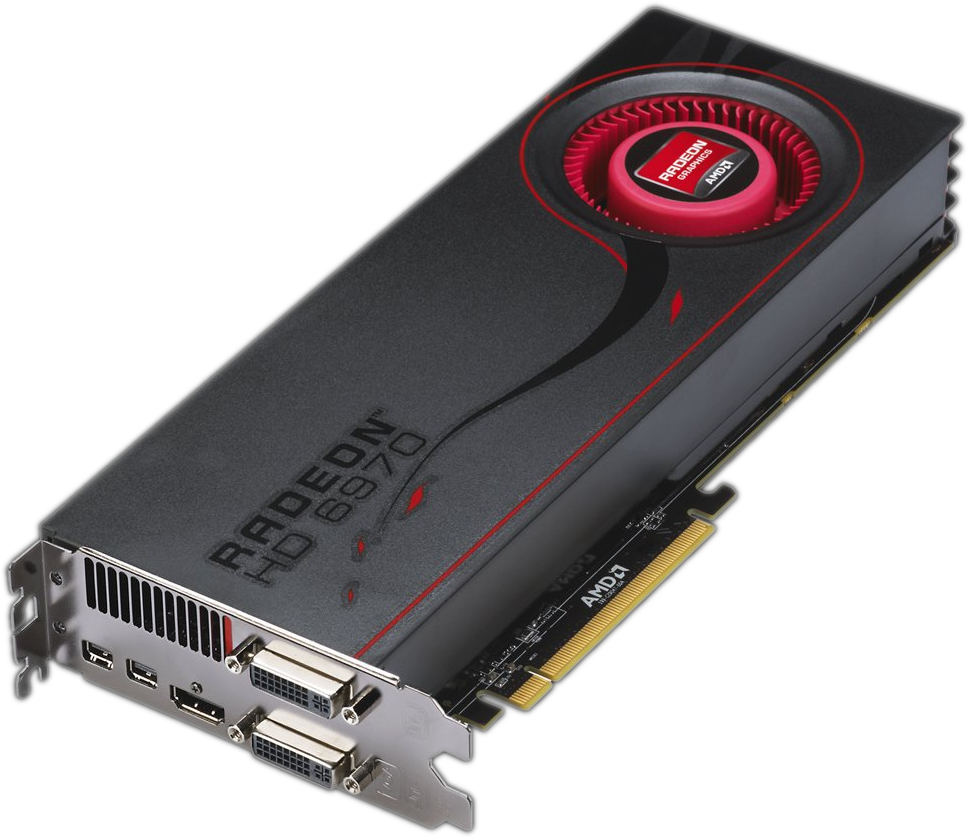
\includegraphics[width=0.6\columnwidth]{amd-6970.png}
